\documentclass{beamer}

\usepackage[T1]{fontenc}
\usepackage{url}
\usepackage{hyperref}
\usepackage{graphicx}
\usepackage{minted}
\newminted{clojure}{fontsize=\fontsize{8}{8},linenos,numbersep=3pt}
\newmintinline{clojure}{fontsize=\fontsize{8}{8}}
\newcommand{\code}{\clojureinline}

\usetheme{AnnArbor}

\title{Solving the TTC FIXML Case with FunnyQT}
\author{Tassilo Horn\\
  \href{mailto:horn@uni-koblenz.de}{horn@uni-koblenz.de}}

\begin{document}
\maketitle{}

\section{Task 1: XML to XML Model}

\begin{frame}
  \LARGE
  \begin{center}
    \textbf{Task 1: XML to XML Model}
  \end{center}
\end{frame}

\begin{frame}
  That's a FunnyQT built-in Transformation.
  \begin{center}
    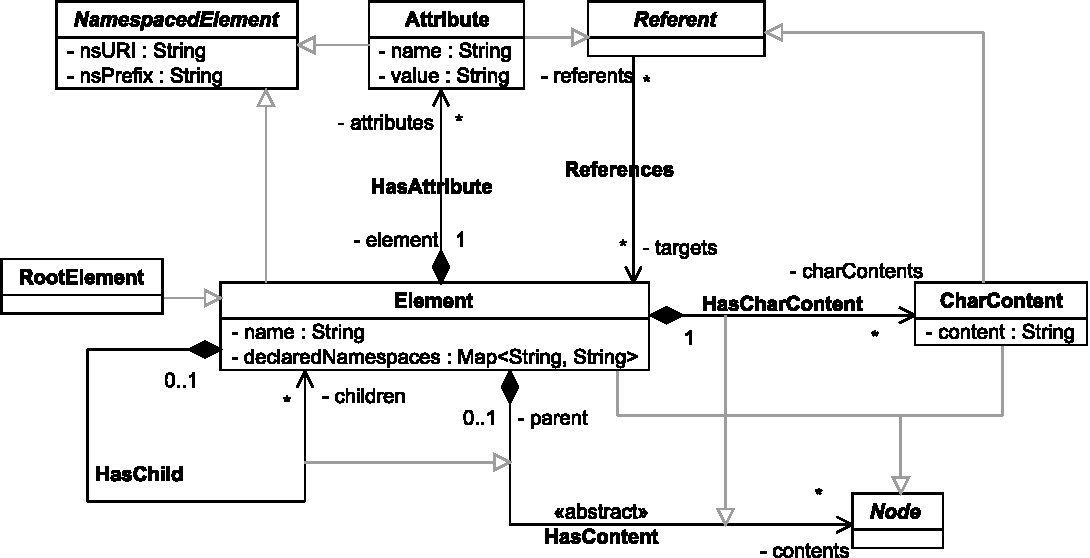
\includegraphics[width=\textwidth]{../doc/xml-schema}
  \end{center}
\end{frame}

\section{Task 2: XML Model to OO Model}

\begin{frame}
  \LARGE
  \begin{center}
    \textbf{Task 2: XML Model to OO Model}
  \end{center}
\end{frame}

\begin{frame}[fragile]
  \frametitle{The OO Metamodel}
  \begin{center}
    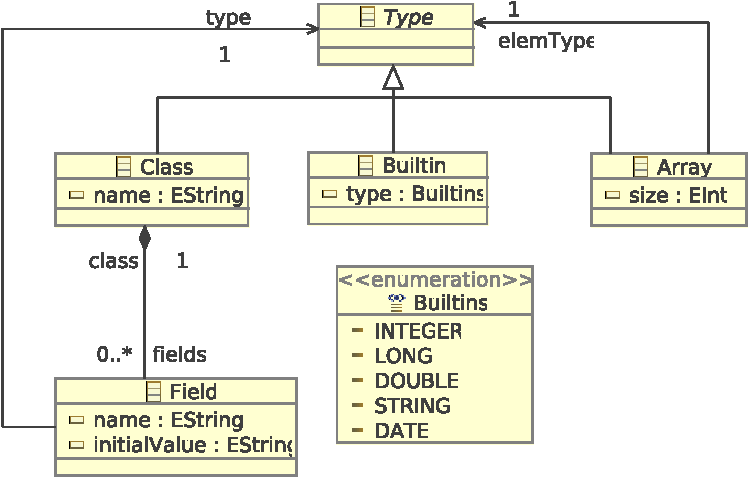
\includegraphics[width=.8\textwidth]{../model/oo.pdf}
  \end{center}
\end{frame}

\begin{frame}[fragile]
  \frametitle{The XML Model to OO Model Transformation}
  \begin{itemize}
  \item Guesses attribute types (integer, long, double, Date, String)
  \item Multiple children of the same name become an array field
  \item Also transforms character contents to fields, e.g.,
    \code|<foo>17</foo>| will become a field of type integer
  \end{itemize}
\end{frame}

\section{Task 3: OO Model to Code}

\begin{frame}
  \LARGE
  \begin{center}
    \textbf{Task 3: OO Model to Code}
  \end{center}
\end{frame}

\begin{frame}
  \frametitle{The OO Model to Code Transformation}
  \begin{enumerate}
  \item Uses the Moustache templating library
  \item Generates Java, C\#, C++, and C code (+ getters, setters, destructors,
    etc.)
  \item Converts OO Model attribute types to what's appropriate in that
    language
  \end{enumerate}
\end{frame}

\begin{frame}[fragile]
  \frametitle{Mustache}
  \begin{clojurecode*}{fontsize=\tiny}
class {{{class-name}}} {
    {{#fields}}
    private {{{field-type}}} {{{field-name}}};
    {{/fields}}

    public {{{class-name}}}() {
        {{#fields}}
        this.{{{field-name}}} = {{{field-value-exp}}};
        {{/fields}}
    }

    public {{{class-name}}}({{#fields}}{{^first}}, {{/first}}{{{field-type}}} {{{field-name}}}{{/fields}}) {
        {{#fields}}
        this.{{{field-name}}} = {{{field-name}}};
        {{/fields}}
    }

    {{#fields}}
    public {{{field-type}}} get{{{field-name}}}() {
        return {{{field-name}}};
    }

    public void set{{{field-name}}}({{{field-type}}} {{{field-name}}}) {
        this.{{{field-name}}} = {{{field-name}}};
    }
    {{/fields}}
}
  \end{clojurecode*}
\end{frame}

\begin{frame}[fragile]
  \frametitle{Mustache}
  \begin{clojurecode*}{fontsize=\tiny}
class {{{class-name}}} {
    {{#fields}}
    private {{{field-type}}} {{{field-name}}};
    {{/fields}}

    public {{{class-name}}}() {
        {{#fields}}
        this.{{{field-name}}} = {{{field-value-exp}}};
        {{/fields}}
    }

    public {{{class-name}}}({{#fields}}{{^first}}, {{/first}}{{{field-type}}} {{{field-name}}}{{/fields}}) {
        {{#fields}}
        this.{{{field-name}}} = {{{field-name}}};
        {{/fields}}
    }

    {{#fields}}
    public {{{field-type}}} get{{{field-name}}}() {
        return {{{field-name}}};
    }

    public void set{{{field-name}}}({{{field-type}}} {{{field-name}}}) {
        this.{{{field-name}}} = {{{field-name}}};
    }
    {{/fields}}
}
  \end{clojurecode*}
\end{frame}

\section{Evaluation and Conclusion}

\begin{frame}
  \frametitle{Evaluation}
  \begin{description}
  \item[Complexity] About 300 expressions, 24 metamodel type references, and 18
    property references
  \item[Accuracy] 100\%
  \item[Dev. Effort] About 12 person hours
  \item[Fault Tol.] Rejects incorrect XML; can reject invalid FIXML if DTD or
    XSD is provided (standard StAX parser)
  \item[Exec. Time] Less than 1 sec for any provided model; 1.6 sec for all 6
    valid models + 5 extra ones in ``multi-message mode''
  \item[Modularity]
    \begin{itemize}
    \item xml-graph2oo-model: 6 rules, 5 dependencies => 0.1666
    \item to-moustache: 10 functions, 12 dependencies => -0.2
    \end{itemize}
  \item[Abstr. Level] medium
  \end{description}
\end{frame}

\begin{frame}
  \frametitle{Conclusion}
  \begin{itemize}
  \item The solution does all extension tasks (except FIXML Schema to Code)
  \item It even does more than the extensions (e.g., destructors, separation in
    header/impl for C++ and C, correct imports/includes, array fields instead
    of multiple fields)
  \item The generated code compiles as-is (without warnings)
  \item It has a more accurate ``multi-messages mode''
  \item It's reasonable fast
  \end{itemize}
\end{frame}

\end{document}


%%% Local Variables:
%%% mode: latex
%%% TeX-master: t
%%% TeX-engine: pdflatex-shell-escape
%%% End:
